\begin{appendices}
\makeatletter
\renewcommand{\thesubsection}{\@arabic\c@subsection}  % label with numbers instead of letters
\makeatother

\subsection{Questionnaire}

A static print of the online questionnaire used in the study is found below.
Minor aesthetic differences are present due to conversion from a web-page,
but all content is identical.

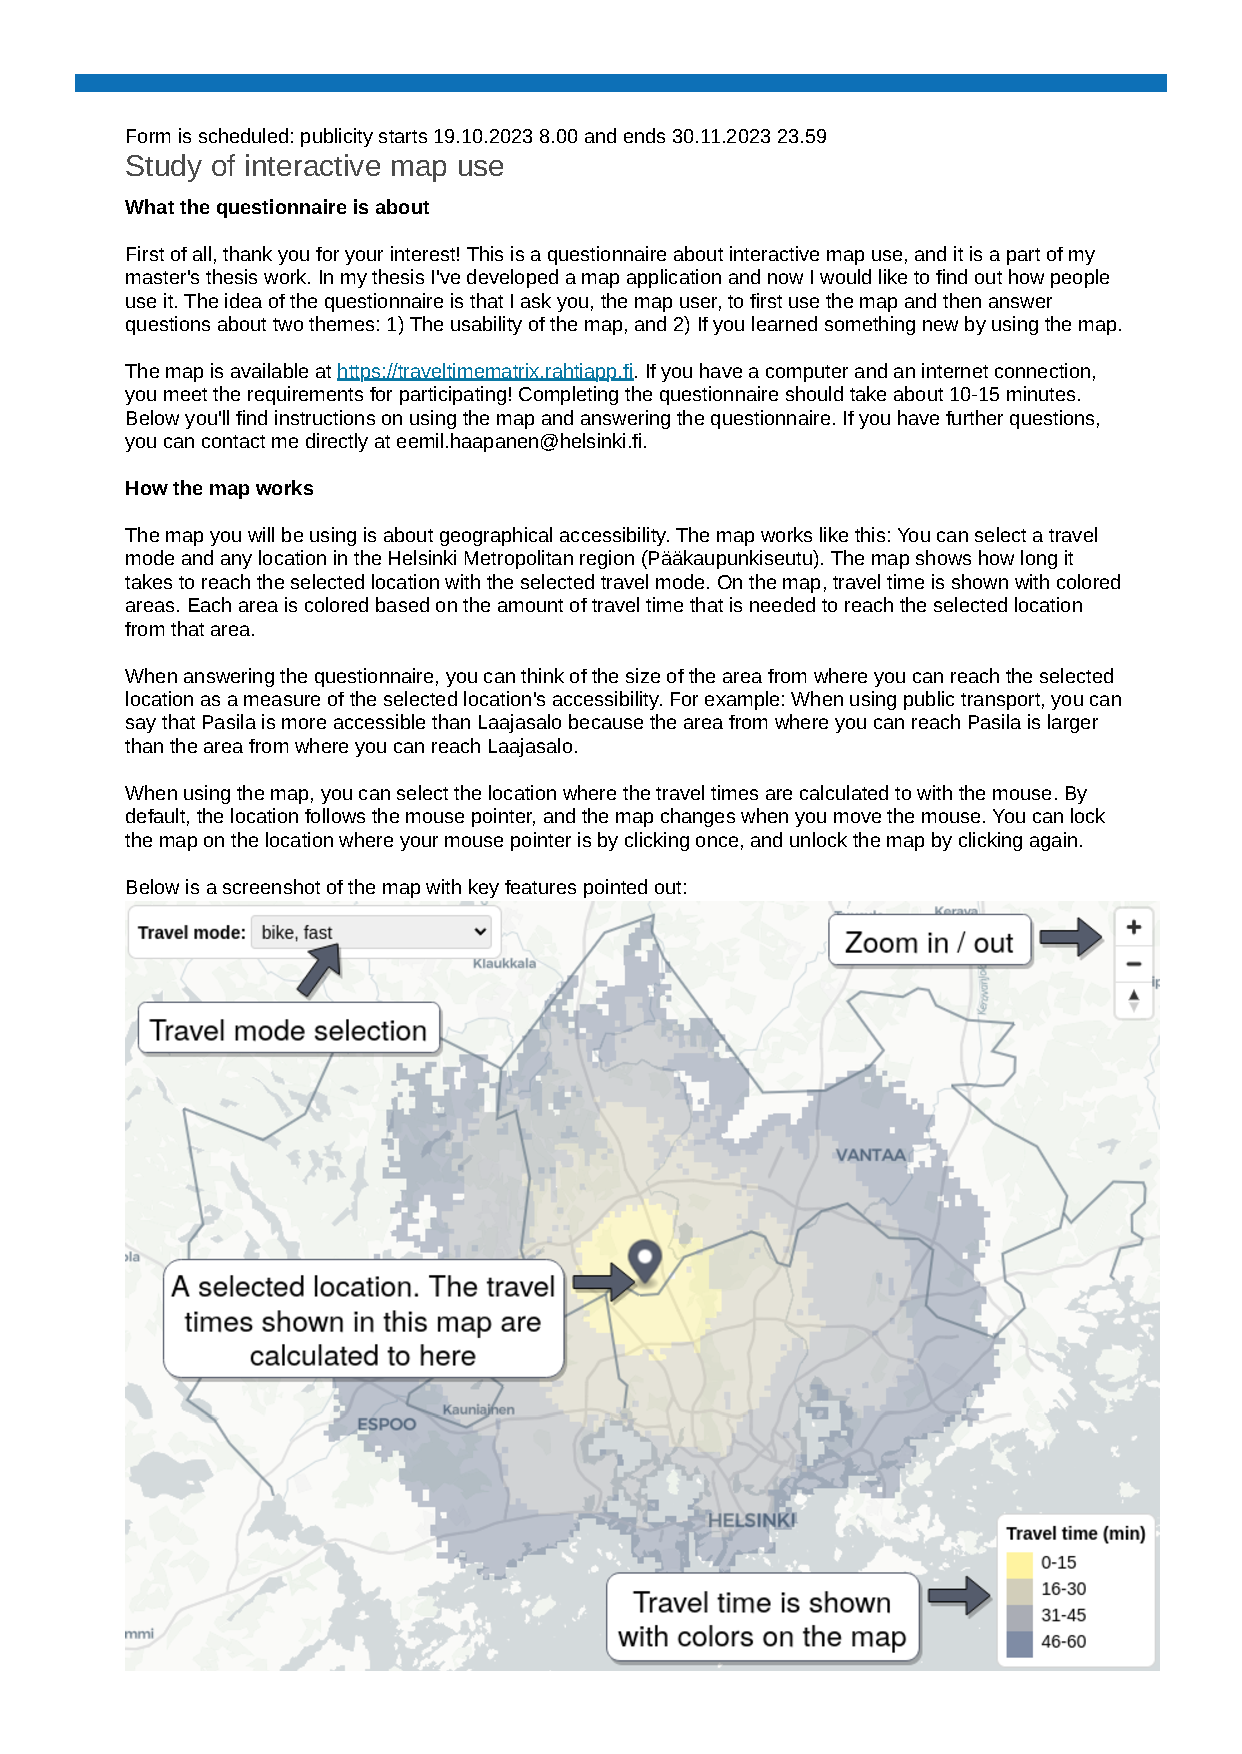
\includepdf[pages={1-},scale=0.9,pagecommand={}]{external_pdf/questionnaire.pdf}

\subsection{Questionnaire responses}

Responses to the questionnaire are presented here.
They are divided into the same task groupings that were used in the questionnaire.

\begin{figure}[H]
	% \centering
	\begin{subfigure}[b]{0.5\textwidth}
	% 	\centering
		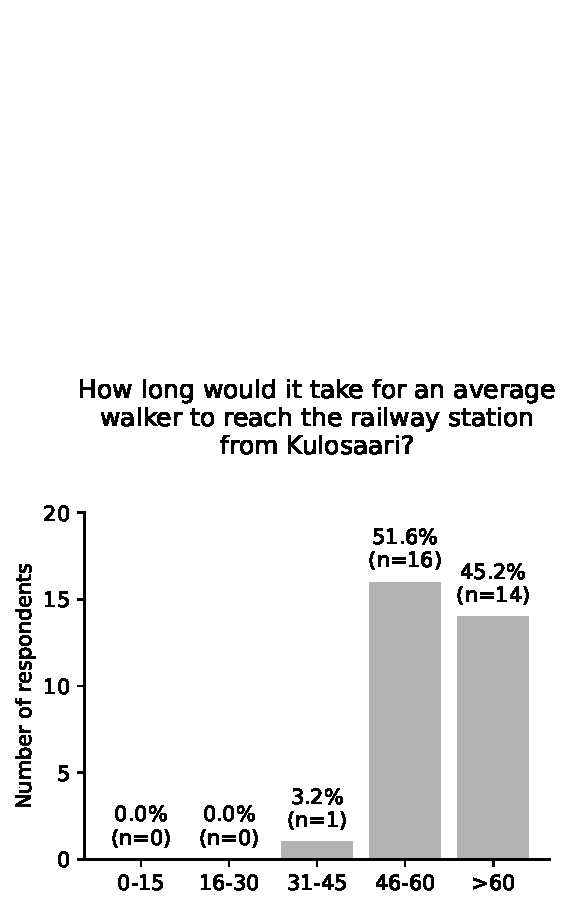
\includegraphics[width=\textwidth]{visual/figures/survey/0.pdf}
	\end{subfigure}%
	\hfill
	\begin{subfigure}[b]{0.5\textwidth}
	% 	\centering
		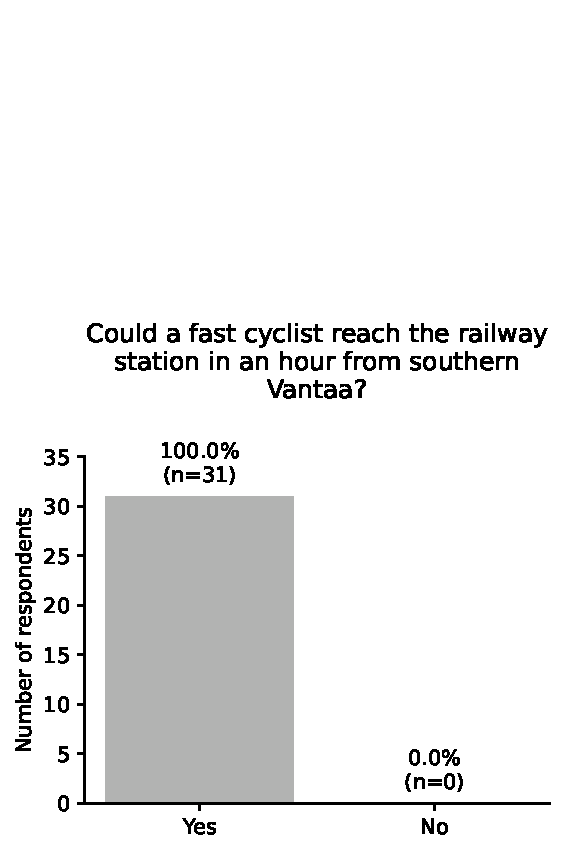
\includegraphics[width=\textwidth]{visual/figures/survey/1.pdf}
	\end{subfigure}%
	% \caption{Responses to task 1}
	% \label{fig:task 1}
	\newline
	Responses to task 1
\end{figure}

\begin{figure}[H]
	% \centering
	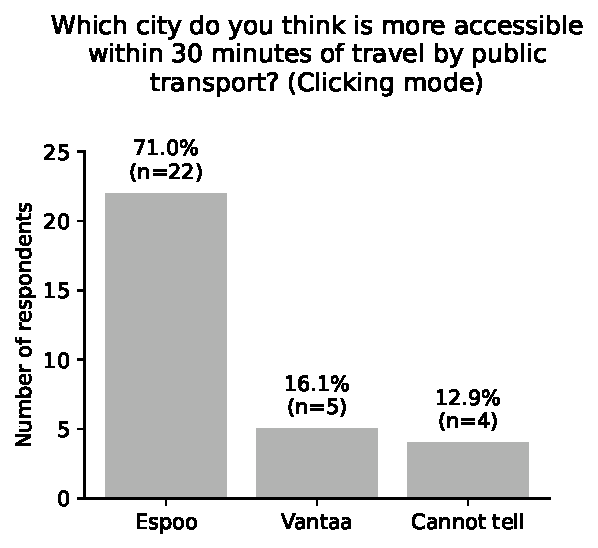
\includegraphics[width=0.5\textwidth]{visual/figures/survey/2.pdf}
	% \caption{Responses to task 2}
	% \label{fig:task 2}
	\newline
	Responses to task 2
\end{figure}

\begin{figure}[H]
	% \centering
	\begin{subfigure}[b]{0.5\textwidth}
	% 	\centering
		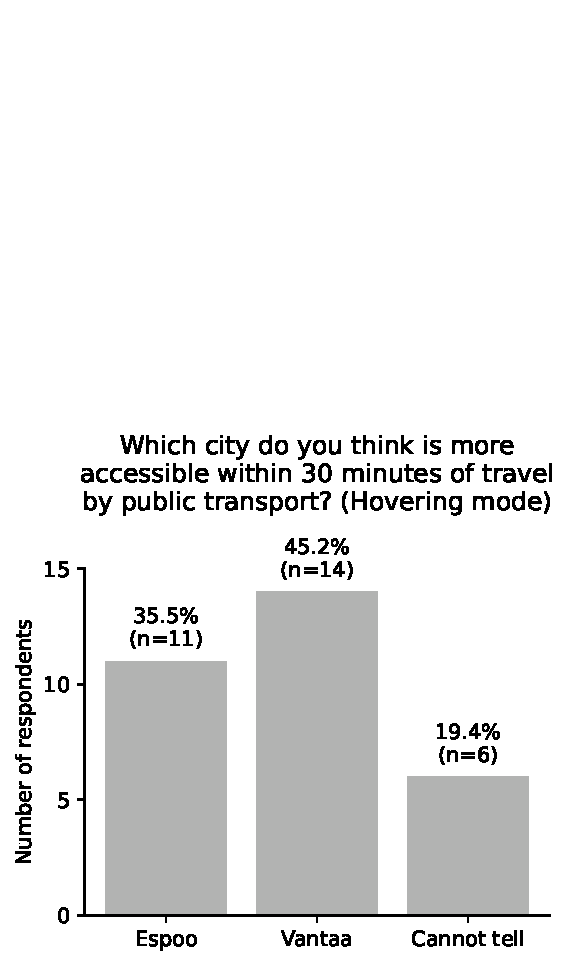
\includegraphics[width=\textwidth]{visual/figures/survey/3.pdf}
	\end{subfigure}%
	\hfill
	\begin{subfigure}[b]{0.5\textwidth}
	% 	\centering
		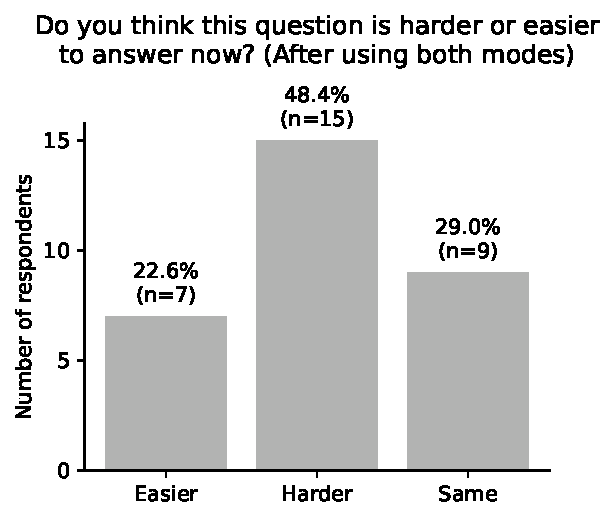
\includegraphics[width=\textwidth]{visual/figures/survey/4.pdf}
	\end{subfigure}%
	% \caption{Responses to task 3}
	% \label{fig:task 3}
	\newline
	Responses to task 3
\end{figure}

\begin{figure}[H]
	% \centering
	\begin{subfigure}[b]{0.5\textwidth}
	% 	\centering
		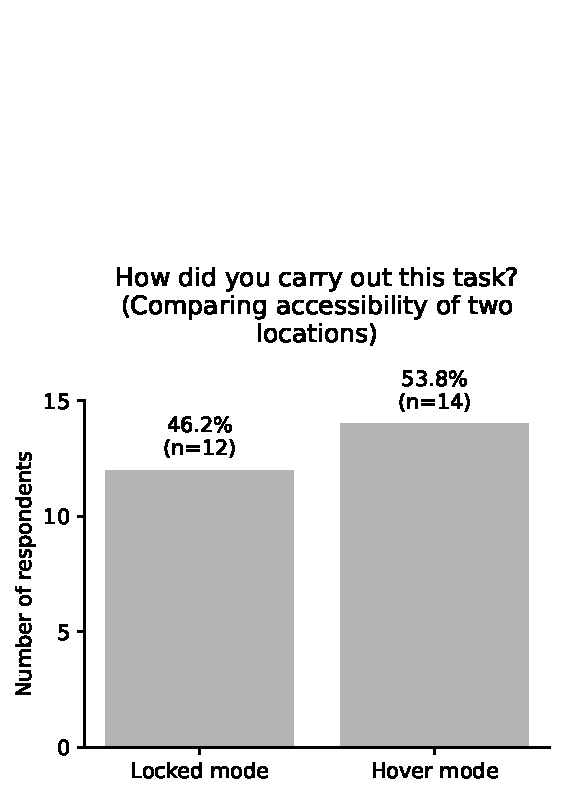
\includegraphics[width=\textwidth]{visual/figures/survey/5.pdf}
	% 	\caption{Responses to task 4}
	% 	\label{fig:task 4}
	\end{subfigure}%
	\begin{subfigure}[b]{0.5\textwidth}
	% 	\centering
		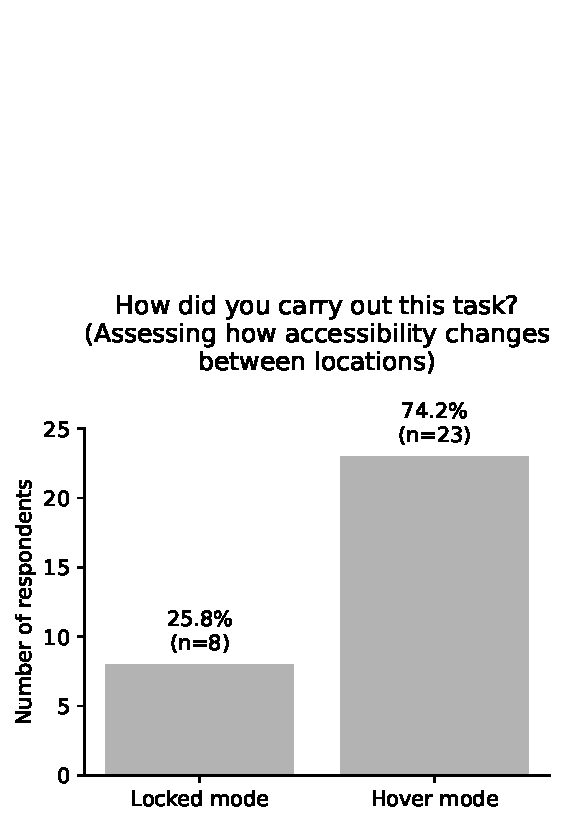
\includegraphics[width=\textwidth]{visual/figures/survey/6.pdf}
	% 	\caption{Responses to task 5}
	% 	\label{fig:task 5}
	\end{subfigure}
	\newline
	Responses to task 4
\end{figure}

\begin{figure}[H]
	% \centering
	\begin{subfigure}[b]{0.5\textwidth}
	% 	\centering
		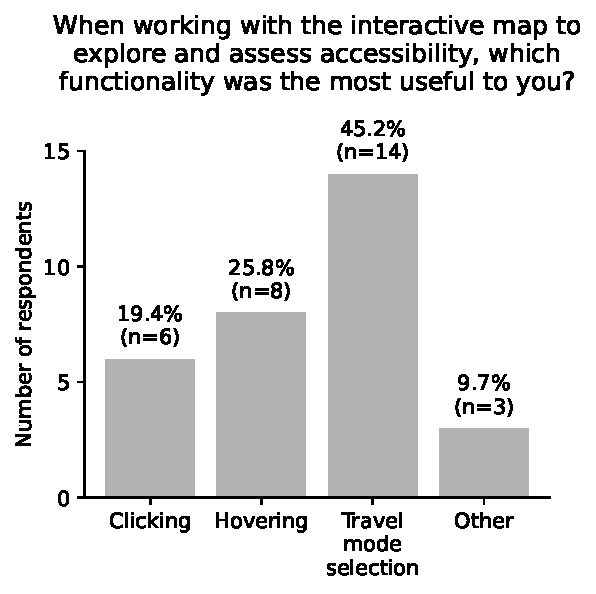
\includegraphics[width=\textwidth]{visual/figures/survey/7.pdf}
	\end{subfigure}%
	\hfill
	\begin{subfigure}[b]{0.5\textwidth}
	% 	\centering
		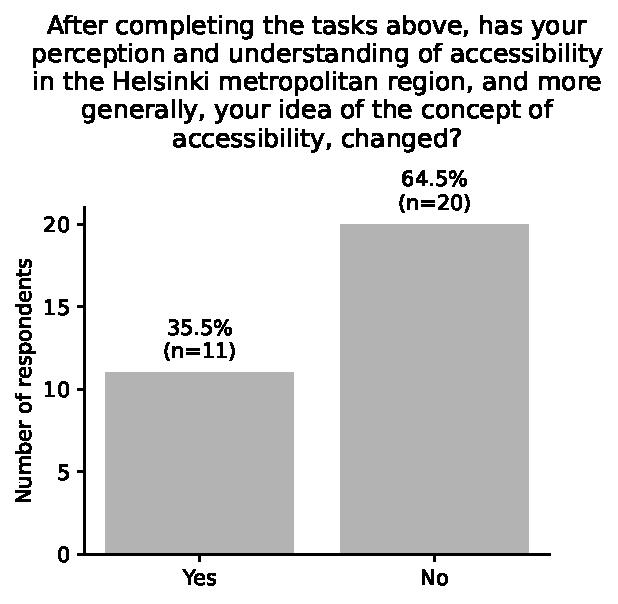
\includegraphics[width=\textwidth]{visual/figures/survey/8.pdf}
	\end{subfigure}%
	\newline
	\begin{subfigure}[b]{0.5\textwidth}
	% 	\centering
		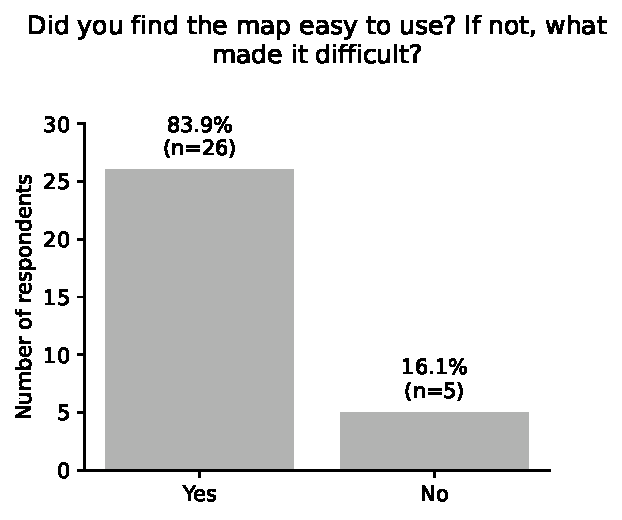
\includegraphics[width=\textwidth]{visual/figures/survey/9.pdf}
	\end{subfigure}%
	% \caption{Responses to general questions}
	% \label{fig:general questions}
	\newline
	Responses to task 5
\end{figure}

\begin{figure}[H]
	% \centering
	\begin{subfigure}[b]{0.5\textwidth}
	% 	\centering
		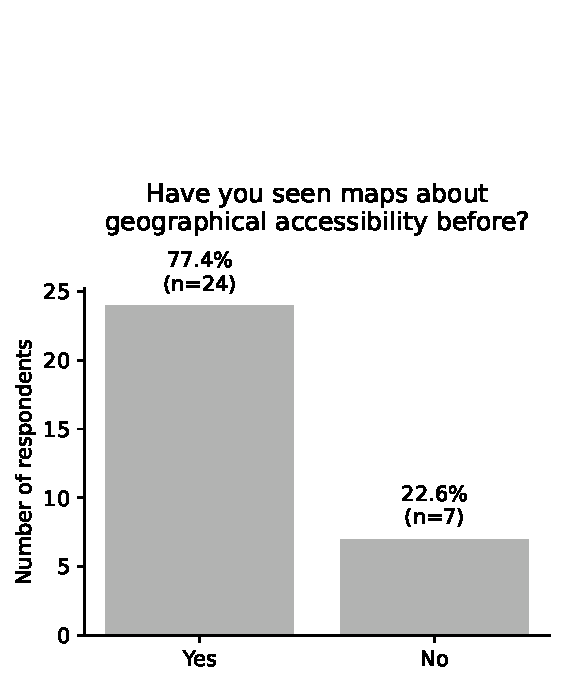
\includegraphics[width=\textwidth]{visual/figures/survey/10.pdf}
	\end{subfigure}%
	\hfill
	\begin{subfigure}[b]{0.5\textwidth}
	% 	\centering
		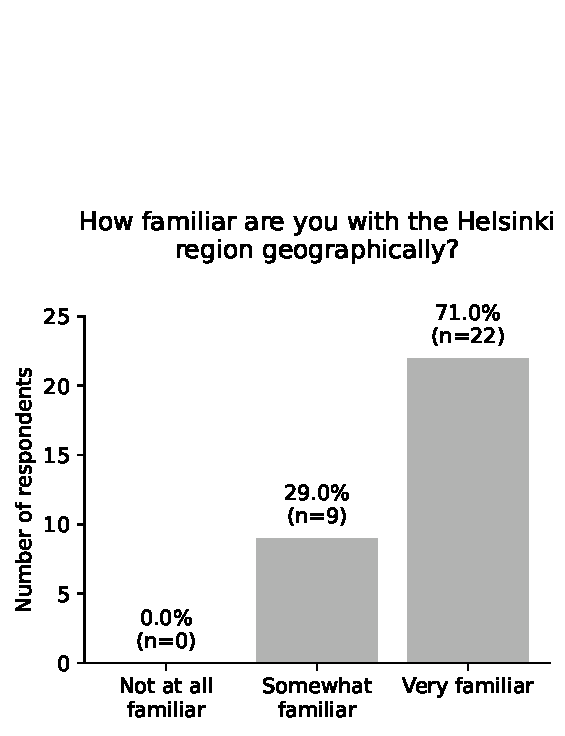
\includegraphics[width=\textwidth]{visual/figures/survey/11.pdf}
	\end{subfigure}%
	\newline
	\begin{subfigure}[b]{0.5\textwidth}  % [t] to position to top
	% 	\centering
		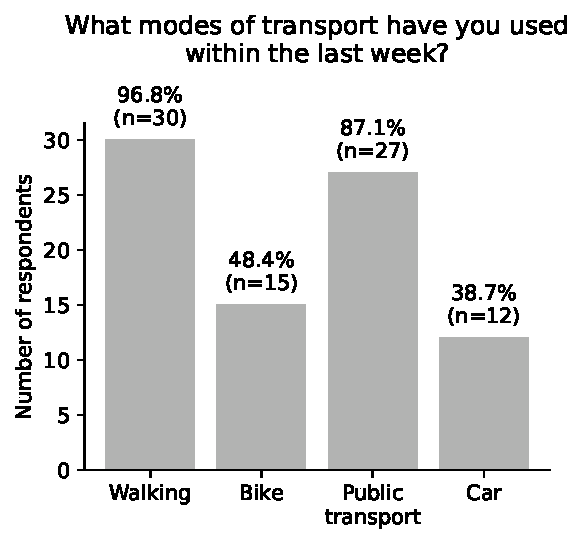
\includegraphics[width=\textwidth]{visual/figures/survey/modes.pdf}
	\end{subfigure}%
	\begin{subfigure}[b]{0.5\textwidth}
	% 	\centering
		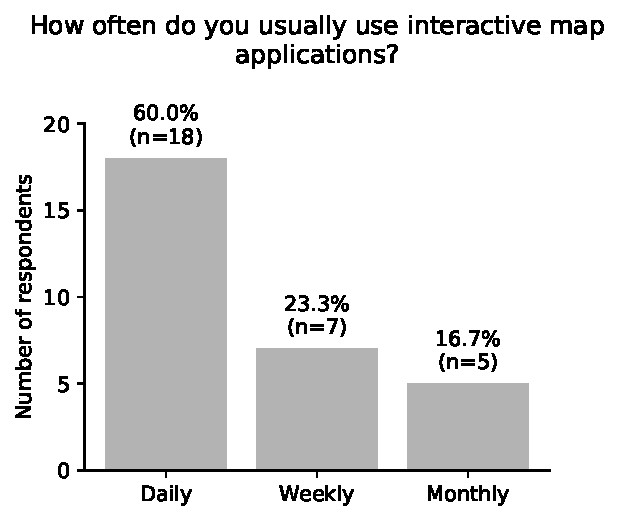
\includegraphics[width=\textwidth]{visual/figures/survey/12.pdf}
	\end{subfigure}%
	% \caption{Responses to questions about background information}
	% \label{fig:background information}
	\newline
	Responses to general questions
\end{figure}

\begin{figure}[H]
	% \centering
	\begin{subfigure}[b]{0.5\textwidth}
	% 	\centering
		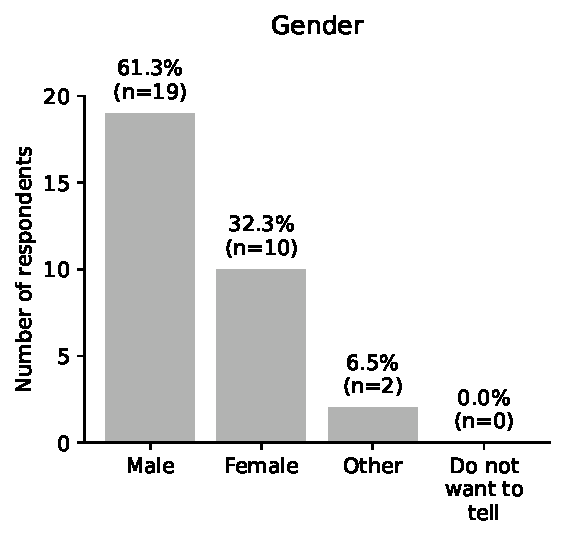
\includegraphics[width=\textwidth]{visual/figures/survey/13.pdf}
	\end{subfigure}%
	\hfill
	\begin{subfigure}[b]{0.5\textwidth}
	% 	\centering
		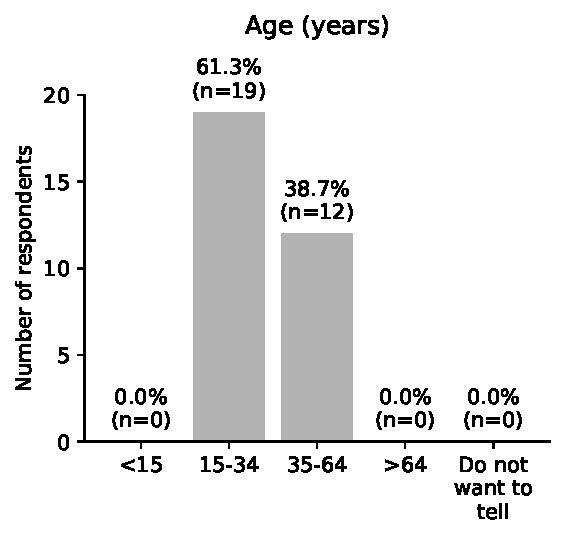
\includegraphics[width=\textwidth]{visual/figures/survey/14.pdf}
	\end{subfigure}%
	% \caption{Responses to questions about demographic information}
	% \label{fig:demographic questions}
	\newline
	Responses to questions about background information
\end{figure}

\subsection{Code repositories}

The source code of all components of the technical implementation
can be found in the repositories linked below.
In addition to code, each repository also includes
the necessary documentation,
dependencies and, when applicable,
development and production environments along with deployment manifests
to develop, run and deploy the components.

\begin{table}[H]
	\centering
	\begin{tabular}{ | L{0.38\textwidth} | L{0.62\textwidth} | }
		\hline
		Map application
		& \url{https://github.com/DigitalGeographyLab/travel-time-matrix-visualisation-frontend}
		\\
		\hline
		Backend
		& \url{https://github.com/DigitalGeographyLab/travel-time-matrix-visualisation-backend}
		\\
		\hline
		Data preprocessing scripts
		& \url{https://github.com/DigitalGeographyLab/travel-time-matrix-visualisation-preprocessing}
		\\
		\hline
	\end{tabular}
\end{table}

\end{appendices}
